\section{Introduction}
 In recent years, image fusion has become an important issue in
image processing community. The target of image fusion is to generate a composite image by integrating the complementary information from multiple source images of the same scene. For
an image fusion system, the input source images can be acquired
from either different types of imaging sensors or a sensor whose
optical parameters can be changed, and the output called fused
image will be more suitable for human or machine perception than
any individual source image. Image fusion technique has been
widely employed in many applications such as computer vision,
surveillance, medical imaging, and remote sensing.
\hfill \break

 As shown in fig \ref{fig1} a,b shows the image whose center and boarder are blared respectively and c shows its fused image which contains the total information contain in source image a \& b.
\hfill \break

 I proposed a technique of image fusion based on MST and SR. In MST image is decomposed into band of low pass and high pass based on the decomposition method and sparse representation sparsely represent an image patch by a dictionary matrix. I combine above two method to take advantage in image fusion. Theoretical description of MST and SR will discuss in second chapter.

\begin{figure}[ht] 
  \begin{subfigure}[b]{0.33\linewidth}
    \centering
    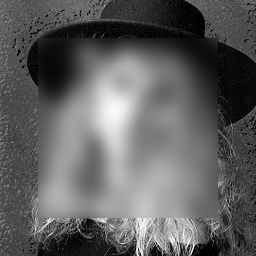
\includegraphics[width=0.5\linewidth]{1a}
    \caption{} 
    \label{1a} 
    \vspace{4ex}
  \end{subfigure}%%
  \begin{subfigure}[b]{0.33\linewidth}
    \centering
    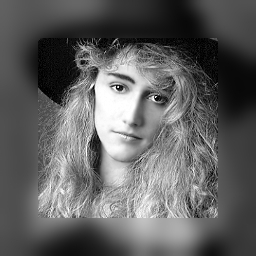
\includegraphics[width=0.5\linewidth]{1b}
    \caption{} 
    \label{1b} 
    \vspace{4ex}
  \end{subfigure}%%
  \begin{subfigure}[b]{0.33\linewidth}
    \centering
    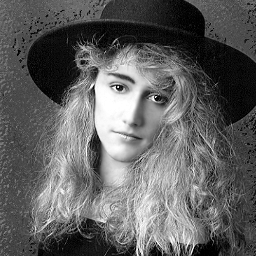
\includegraphics[width=0.5\linewidth]{1c} 
    \caption{} 
    \label{1c} 
    \vspace{4ex}
  \end{subfigure}%%
  
  \caption{(a),(b)Sensor image from two source.(c)Fused image of a,b.}
  \label{fig1} 
\end{figure}

\section{Motivation}
The major, recurrent theme throughout this work is my search for a good fusion model for image fusion of multifocous and natural
images. In addition, I seek a model for image fusion based on sparse representation that is capable of approximating the images with only fewer non zero coefficient. The hope is that I would find out a simple model that can fuse multiple images. Finally, the computation  time for the model would be small and fusing the images would be easy enough.

\section{Problem Statement}\label{sec:ProbStatement}
Being able to fuse multiple image is a very challenging task, but it could have great impact, for instance when taking image by digital camera it focus one object while another in different distance remain blurred or unfocused as shown in figure \ref{fig1.2} .My task is to fuse image from different source sensor and generate an image that is fully focus for every object at relative distance in the fused image.

\begin{figure}[h]
  \centering
  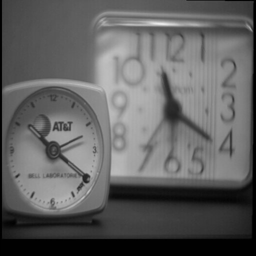
\includegraphics[width=0.5\linewidth]{1d.png}
  \label{fig2}
  \caption{Example of a multifocus image.}
\end{figure}


\section{Objectives}
% List items using bullets

\begin{itemize}
  \item First objective is to find efficient method to fuse images.
  \item Next objective is to remove any artifact produced by fusing transform coefficient. 
  \item To remove noise introduced in source image from fused image.
\end{itemize}


